\startchapter{Implementation}
\label{chapter:imp}

In this chapter, we take a look the implementation of the Sage prototype. We examine each filesystem object in detail and finally look at how Sage is used.

\section{Overview}

SageFS (or Sage) is implemented as a Python client library and is used by importing into a  Python project. I chose to use a client library instead of system component was because a  client library is much easier to use and deploy. Additionally the initial use case for  Sage was for Python applications accessing a large repository of satellite imagery as discussed in the Green  Cities application in Chapter \ref{chapter:intro}.  Once imported, a Sage object can be created to interact with SageFS, which contains a number of translator objects. Currently there are only two types of translators, SwiftTr and MongoTr  that connect with Swift object stores and MongoDB instances respectively. Translators are the components that actually interact with backend stores, and essentially translate filesystem  commands into the appropriate set of commands for the backend storage. For example, when the SageTr object's open method is called on a file in a Swift backend, SageFS call the containing  SwiftFS open which downloads the file and stores it in a SageFile object for use by the application.  SageFile objects are file abstractions built on top of Python files. SageFile objects have two subclasses, namely SageMemFile and SageDiskFile objects. Both have the same functionality, however  SageMemFile objects exist in memory only, while SageDiskFile objects are actually written to disk.  Applications communicate with SageFS directly and through the use of SageFiles. To store files in backend repositories SageFS communicates with translator objects, notably SwiftTr and MongoTr  which actually communicate back to the backend. This way Sage can make multiple backends appear  as a single entity, with a common API. 

One important thing to notice here is that Sage does not go through the OS for
normal operation.  The OS is used for networking and to put opened files on
disk (if they are requested not to  reside in memory). However, if a
translator does not go through the OS, an application that  used the `no OS
translator' could use normal Python file operations and never go through the
OS!


\begin{figure}[h]
\centering
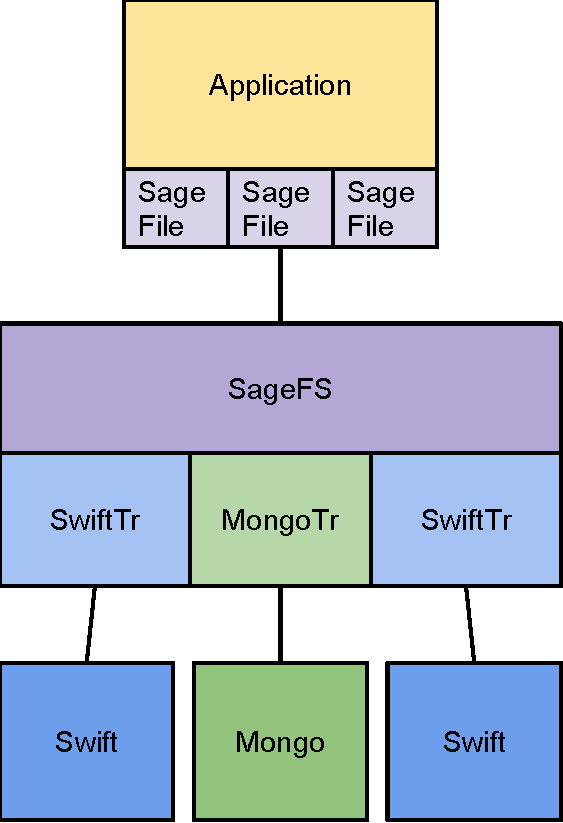
\includegraphics[scale=0.7]{figures/implementation}
\caption[Example Sage Deployment]{An Example of a possible Sage deployment with the current Implementation}
\label{fig:implementation}
\end{figure}


\section{File Objects}

We start looking at the filesystem by examining the actual file objects.
There are two types of Sage file objects, SageMemFile and SageDiskFile.  Both
objects inherit from the SageFile class, but SageMemFile inherits from  the
StringIO class while the SageDiskFile inherits from the base Python file
class. This allows the SageMemFile to reside as a buffer in memory, excellent
for smaller files that are consumed rapidly and do not need to be persisted,
while a SageDiskFile is actually written as a temporary file on the client
system.  The base SageFile object has a few key variables and methods that
facilitate interaction  with Sage. Each SageFile knows which backend
repository it belong to and uses this  in the sync() method which re uploads
the file into the backend. sync() can be called  on its own but it is also
called within the write() family of methods for SageFile  objects. If we take
the write method as an example, we see it takes three arguments.  The first is
a reference to the calling object (Python makes this explicit, while in  a
language like Java the self reference `this' is always the first argument to a
method,  but not explicitly stated in the method signature). The second
argument is the argument  to the underlying file object's write method, while
the third is a flag indicating whether  or not we should sync the file at the
end of the write operation. This is included incase  we only want to update
the local copy and not write back into the backend repository after  every
write (ie. cached writes). The close() method looks similar to write() except
it only  takes the sync argument. When a file is closed it is first synced
back to its backend  repository, then removed from a local filesystem cache
from sage. The file is only removed  if the sync was successful so If an error
occurs, the file will still reside in sage and no  data is lost. A special
method for SageFiles called todisk() will take the file from Sage  and persist
it to the local system. This is a convenience method that allows files to be
easily taken from Sage.

\begin{figure}[h]
\centering
\begin{lstlisting}

def write(self, arg, sync=True):
  """ Calls the underlying write function for the file.
  Will sync with remote storage by default, 
  will not if sync is False """
  self.fileclass.write(self, arg)
  if sync: self.sync()

\end{lstlisting}
\caption{SageFile write function}
\label{fig:sagefilewrite}
\end{figure}

\begin{figure}[h]
\centering
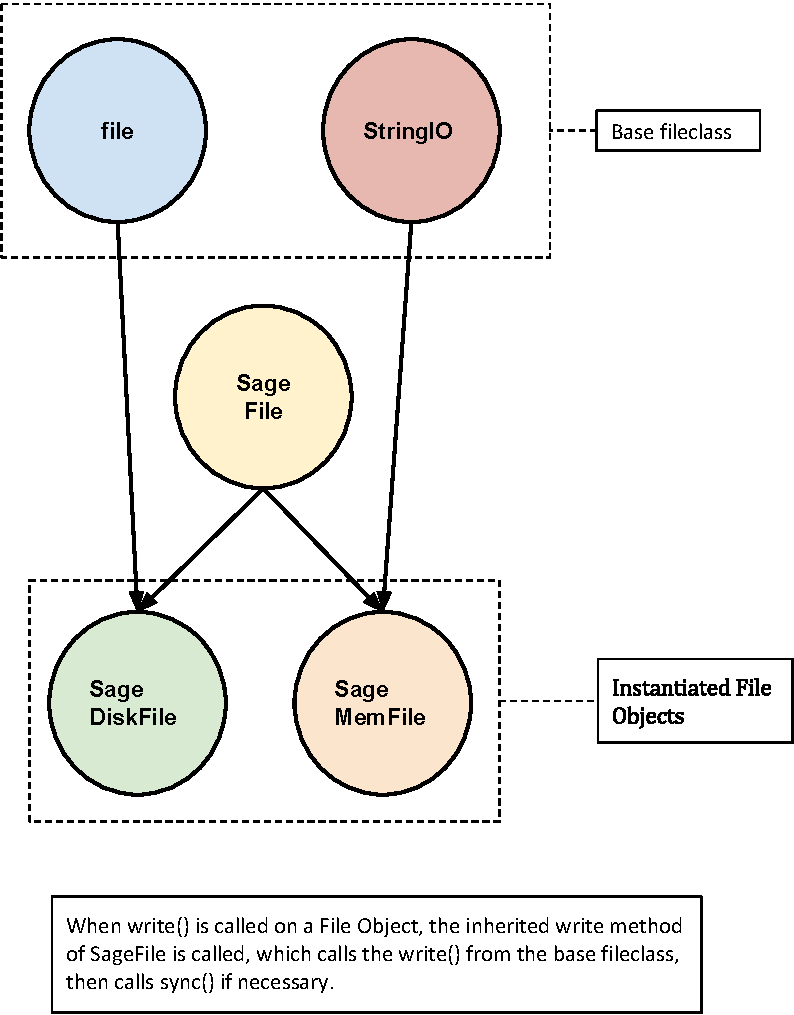
\includegraphics[scale=0.7]{figures/sagefile}
\caption{SageFile inheritance graph}
\label{fig:sagefile}
\end{figure}


\section{Backends}
\label{sec:backends}

Before we examine translator objects lets first take a look at the backend stores that
FS objects actually connect to, and how we can view them as filesystems.

\subsection{Swift}

Swift is an object store system developed by OpenStack as an open source
alternative to Amazon's S3. Clients interact with Swift's RESTful api through
HTTP using PUT and GET to access files. Swift has two main types of nodes,
storage which actually store data, and proxies which handle requests to Swift.
What makes a machine a storage or proxy node depends on the set of processes
running, and in fact a single machine can be both a storage node and a proxy
node. Swift distributes and replicates files across all storage nodes using
what are called `rings'. Figure \ref{fig:swift} shows an object placed
within a Swift cluster. When an object is stored in Swift it is first assigned
to ring, which then handles distribution over a set of storage nodes where it
is stored as a blob. The Proxy node handles the partitioning of the file based
on the ring configuration, then sends data to the storage nodes. The number of
nodes a file is distributed to is called the replication factor for the
storage set. It is worth noting that all requests go through the proxy nodes
(a cluster can have multiple proxies and each request goes to exactly one of
them), so clients never directly contact the storage nodes.

\begin{figure}[h]
\centering
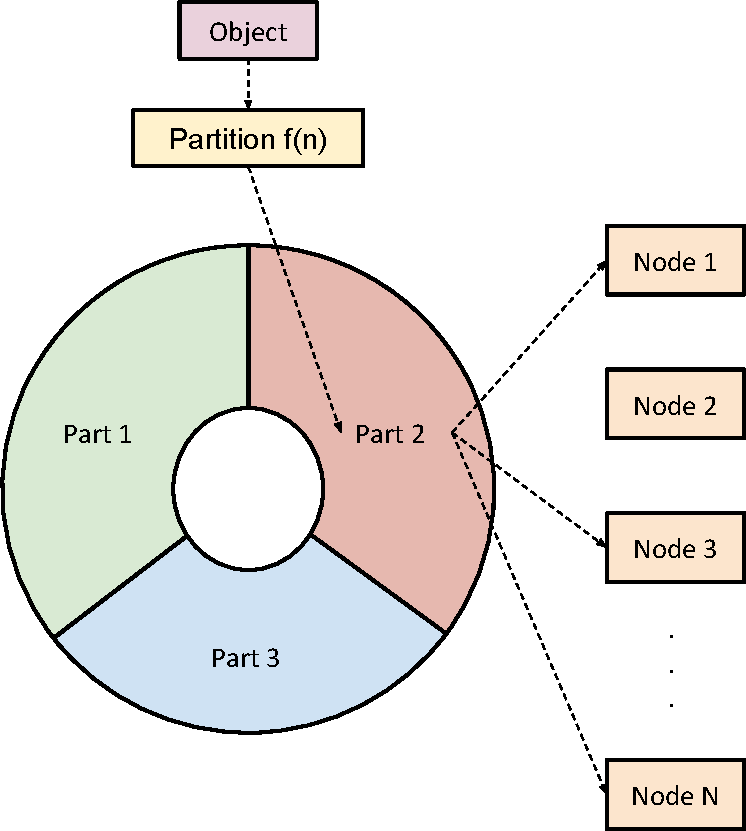
\includegraphics[scale=0.7]{figures/swiftrings}
\caption{The OpenStack Swift Ring Structure}
\label{fig:swift}
\end{figure}

Swift also contains accounts and containers which logically separate files
into groups which I use to implement users and groups in Sage. Each group is
an account and each container is a different user. We could have easily
implemented an account for each user since groups are not implemented in the
filesystem, but using accounts is one way future implementations could. Files
are stored based on their full path so directories do not physically exist,
though Swift can mark a zero byte file to act as a directory. The Swift client
allows partial name matching which we can use to search for all files
logically grouped in a directory by simply querying the path name as a
substring. We use the swiftclient module to communicate with Swift through
Python.

\note{put\_object and get\_object? Also the figure of how users and groups are done}


\subsection{MongoDB}

MongoDB is a NoSql database which stores objects in what is called document
oriented storage. Related documents are organized into collections that allow
efficient querying and indexing. Data is stored as BSON a superset of JSON
that allows Mongo to store arbitrary bytes of data. Mongo can exist as a
standalone database on one machine, or can be distributed in a cluster. When
distributed Mongo has Config Servers which hold metadata, and Shards that
house the data. A given document collection can be distributed across shards
much like disk striping. Config Server metadata is held in a config database
(a single Mongo instance can contain multiple databases) which maps documents
to Shards. Shards contact the Config Servers to access metadata (which Shards
heavily cache). I make use of databases and collections to implement users and
groups, and store files as a key value pair document, with the key being the
full file path, and the value being the files binary data. In the actual
document we store path and file name as two separate fields as we want to be
able to search for paths and partial paths when listing files. We use the
Python module pymongo to communicate with MongoDB.

\note{collection.insert and collection.find\_one ????}


\subsection{Local}

A very rough implementation exists to incorporate the local filesystem into
Sage. This was developed mostly for testing purposes and is missing
functionality other than reading and writing files. Files are created in a
temp directory which acts as the root for the filesystem.


\section{Translator Objects}

Translator objects in general must implement upload() open() stat() copy()
move() list() and remove() methods as SageFS hands off functionality to the
translator objects when performing filesystem operations. Additionally the
translator must keep a list of files opened with it that have not been closed.
The open() call is one of the only calls that can change the state of the
filesystem as it opens a file descriptor within the system. open() is actually
called on the SageFS object which then calls the underlying translators open()
passing the arguments through. We visit the SageFS object later in the
section. As we can see from the method signature in Figure \ref{fig:sagefsopen}
the open() call has one required parameter and two optional, create which
defaults to false and inmem which defaults true. If the file specified at path
does not exists in the repository and create is true then an empty file will
be created for the translator to keep track of. The file is not actually
created in the backend until it's sync() method is called. The second argument
specifies whether the file should reside in memory or on disk on the local
system. If inmem is true then the file is opened as an SageMemFile, otherwise
it is opened as a SageDiskFile. If open is called on an already open file, the
translator returns the open file descriptor for the file instead of a new file
descriptor for the file. This is done to avoid consistency issues to do with
having two sets of the same file downloaded. It would be possible to implement
file pointers within the SageFile object to allow having two file descriptors
for the same file, but this functionality does not exist in the current
implementation.


\begin{figure}[h]
\begin{lstlisting}

def open(self, path, create=False, inmem=True, *args):

\end{lstlisting}
\caption{The SageFS API's open method signature}
\label{fig:sagefsopen}
\end{figure}

The rest of the translator is convenience methods or methods for connecting to
the backend repository. For example SwiftFS is an object that holds all the
relevant info to connect to swift as well as interface back with SageFS. The
actual Swift repository knows nothing about the front end translator and
communicates via the RESTful interface provided. This makes implementing translators
simple since the six methods just have to be translated into the appropriate
REST calls. The translator also converts filesystem paths into actual
locations in the backend store. Since both Swift and MongoDB are not natural
filesystems we have to fake paths and folders within them. To do this we
simply incorporate the full path as the actual name of the file in the backend
store. This allows the filesystem to logically separate files into a virtual
directory tree, and query based on a fragment of the path. Both Swift and
MongoDB have partial querying built in, but if a backend store was used that
did not have such functionality, then the translator would have to query every
file in the backend and filter the results in the client which could have a
large performance impact.


\section{SageFS}

The SageFS object is the central component of the filesystem and implements
the API (the seven methods  open(), remove(), list(), stat(), copy(), move(),
and upload()) exported for use by applications. Of course an application could
use any part of the sagefs.py Python module, but the intended use is to
interact with the SageFS object. The SageFS object holds a dictionary mapping
names to translator objects as well as a list of all the available backend
repositories, called sites, to the Sage instance. The SageFS constructer and
connect\_to\_filesystem methods are shown in Figure \ref{fig:sagefscode}. The
actual translator objects are not instantiated until the site is actually
used. When a site is accessed the connect\_to\_filesystem() method is called
which creates an translator object and stores the object in the filesystems
dictionary. If more backends were to be added the connect\_to\_filesystem()
method would need to be modified to handle creation of the filesystem objects,
and the constructor for SageFS would need to store a new list for the new
backend repository type. This approach is not the most scaleable so if many
new types of filesystems were to be added, the constructor should take a
dictionary of site names and the constructor method of the appropriate
backend. This way connect\_to\_filesystem() can index into the new dictionary
and call the translator constructor without going through a long chain of
if/else statements.


\begin{figure}[h]
\begin{lstlisting}

class SageFS():
  """ The main filesystem object which holds a collection of SwiftFS
  and MongoFS objects. Connections are only established when they
  are used the first time. The SageFS object is designed to be the 
  only object that must be explicitly created to use the SageFS. """

  def __init__(self, swiftrepos=hosts.swift, mongorepos=hosts.mongo):
    self.filesystems = {}
    self.swiftrepos = swiftrepos
    self.mongorepos = mongorepos
    self.sites = self.swiftrepos.keys() + self.mongorepos.keys()

  def connect_to_filesystem(self, site):
    """ Creates a translator object if we correctly connected """
    fs = None
    if site in self.swiftrepos.keys():
      repo = self.swiftrepos[site]
      fs = SwiftFS(repo.get_authv1_url(), repo.group, repo.user, repo.key)
    elif site in self.mongorepos.keys():
      repo = self.mongorepos[site]
      fs = MongoFS(repo.host, repo.port, repo.database, repo.collection)
    else: raise SageFSException('No host matches site %s' % (site))
    self.filesystems[site] = fs
    return fs

\end{lstlisting}
\caption[SageFS Constructor]{The SageFS constructor and connect\_to\_filesystem methods. The class instance variable self.filesystems holds the SageFS objects collection of translators.}
\label{fig:sagefscode}
\end{figure}


From a high level, when a method is called on the SageFS object the method
first chooses the correct translator based on the file placement logic, then calls the
underlying translators method to perform the call. In the current stable
implementation of placement logic is done by path name via the method
split\_location\_from\_path() (which is easily extended as discussed in section
\ref{chapter:conc}). The method returns an index into SageFSs filesystem
dictionary, which is then used to grab the appropriate translator to perform the
operation on. Some operations operate over a set of translators, stat() and list() can
be used to probe all the translators, while copy and move may involve two different
filesystems. To get a better understanding of how the components work together
in SageFS let us examine the copy() method, shown in Figure \ref{fig:sagecopy}, as while it is the most
complicated, it demonstrates the power of the aggregation of multiple translators in
SageFS.

\begin{figure}[h]
\begin{lstlisting}

def copy(self, origpath, newpath, overwrite=False):
  """ Copy a file from 'origpath' to 'newpath'.
  Will not overwrite unless specified """
  if origpath == newpath: return
  origlocation, origresource = self.split_location_from_path(origpath)
  newlocation, newresource = self.split_location_from_path(newpath)
  origfs = self.get_filesystem(origlocation)
  if origlocation == newlocation:
    # if both resources use the same fs use the fs's copy
    origfs.copy(origresource, newresource, overwrite)
    return
  newfs = self.get_filesystem(newlocation)
  # check to see if we are overwriting anything
  if not overwrite and newfs.file_exists(newresource):
    raise SageFSFileExistsException('File %s already exists' % (newpath))
  local = True
  if origresource not in origfs.localfiles:
    # make sure the orig file is local to its fs
    local = False
    origfs.open(origresource)
  origfd = origfs.localfiles[origresource]
  # upload as a new resource
  try: newfs.upload(newresource, origfd)
  except swiftclient.client.ClientException as e:
    raise SageFSException('HTTP Error: %s - %s' 
               % (e.http_status, e.http_reason))
  if not local: origfd.close() 

\end{lstlisting}
\caption{The SageFS API copy method}
\label{fig:sagecopy}
\end{figure}

The method takes three arguments, origpath which is the path to the original
file to copy, newpath which is the desired path to the new copy of the file,
and an optional argument overwrite which specifies whether the newpath should
overwrite an existing file if it exists. First the method checks if we are
trying to copy to the same location to avoid redundant work, if we actually
need to copy then we determine which filesystems the old file and new file
belong to (or should belong to). If the copies will reside in the same
filesystem we then delegate the work to be done by the translator object, and pass
along the arguments. If they will not reside in the same translator we first check if
we should overwrite the new location and if so, that a file does not exist at
that location. If either of the above is true then we raise an exception
saying that the file already exists. Next we check to see if the SageFile is
open in the original files translator. If it does not then we must open the file so we
can copy it and we also want to remember the file was not open at the start of
the call so we set the variable local to false. We then call upload on the new
translator, giving the new file name and the old files data as arguments. This makes a
copy of the file in the new filesystem without actually opening the file which
ensures the set of open files in the new translator remains unchanged. We finally
close the original file if it was not local to the original translator as again we
want the set of open files to remain unchanged.


\section{Configuration}

SageFS takes a collection of repositories as arguments, which can either be
passed to the constructor or defined in the configuration file hosts.py in the
sagefs python package. The configuration is a dictionary of Host objects in
this case SwiftHosts and MongoHosts. These objects define connection
parameters to each of the backends including username, hostname, and the key
which will identify the filesystem. As an example Figure \ref{fig:swiftconfig}
shows a configuration dictionary for Swift filesystems and is the dictionary
that is passed by default to the SageFS constructor previously shown in Figure
\ref{fig:sagefscode}. The dictionary contains three entries vic, tor, and carl that
map to three SwiftHost objects which simply define parameters to connect to a
Swift repository. Here we see the IP addresses of three Swift installations
that are used as backends and are actually used in the deployment of SageFS
for the genome searching case study described in Chapter \ref{chapter:exp}. To
add or remove filesystems to Sage the we can simply modify the dictionaries in
the configuration file with the appropriate connection parameters, or simply
pass in our own dictionary to a SageFS object.


\begin{figure}[h]
\begin{lstlisting}

swift = {
  'vic':SwiftHost('142.104.17.135', 'admin', 'system', 'sagefs'),
  'tor':SwiftHost('142.150.208.220', 'admin', 'system', 'sagefs'),
  'carl':SwiftHost('134.117.57.138', 'admin', 'system', 'sagefs')
}

\end{lstlisting}
\caption{Configuration dictionary for Swift backends}
\label{fig:swiftconfig}
\end{figure}

Currently, the SwiftHost and MongoHost objects are the only SageHost objects
defined in hosts.py. SwiftHosts require a hostname (or IP address), user,
group, and key to connect to a Swift backend, while MongoHosts require a
hostname, database name, and collection name. Section \ref{sec:backends}


\section{Using Sage}

To use Sage from a client perspective we only needs to import the sagefs
Python module into their Python project. This will allow us to use SageFS with
the default filesystems and defult user provided in the hosts.py configuration
file. To use different filesystems we can either modify hosts.py or pass in
our own dictionary containing the desired filesystems. One thing to note is
that if we define a filesystem that does not exist or does not accept the
connection parameters we provided, SageFS will not fail until we try and
access the dysfunctional filesystem. We can also define a filesystem twice
with a different dictionary key. SageFS will think the two filesystems are
different and allow file operations on both. If we open the same file in both
filesystems two copies of the same file will exist on our machine and if we
write different things to each copy, the copy with the last sync() operation
will be what appears in the backend (If the backend has no file locking!).
This implies that SageFS does no file locking and leaves it up to the backend
store as discussed in Chapter \ref{chapter:arch}.

\begin{figure}[h]
\begin{lstlisting}

import sagefs
fs = sagefs.SageFS()
__builtins__.open = fs.open

\end{lstlisting}
\caption[SageFS Open Hack]{An interesting hack to overwrite Pythons builtin open call to use Sage's instead.}
\label{fig:sagepythonhack}
\end{figure}

Once the module has been imported we create a SageFS object which allows us to
perform operations on the filesystem. To interact with files we call the
SageFS objects open() which returns a SageFile object, which is then used
normally like any other Python file object. In fact if we were to modify an
existing python project to use Sage we would only need to import the sagefs
module, then instantiate a global filesystem object and overwrite the built in
open() function with our filesystems open(). After doing this all calls to
open will go through Sage and all file objects will be SageFiles and will work
without further modification. We could also go a step further and define a
closure around Sages open to extract information about the file and pass it to
open() to allow interesting file placements! Of course other operations from
other modules that utilize the built in open() or modules that manipulate the
local filesystem will remain unchanged so more work may be required on a more
complicated system. Additionally Sages open() will throw different exceptions
than the built in so applications would suffer from unexpected errors if one
occurred.

The client side of SageFS is implemented as a python package which can be
downloaded from github. I also developed server side deployment scripts for
Swift, which will install and configure Swift on a cluster of machines (either
Ubuntu or Fedora) using the Fabric Python module. Once the Swift cluster (or
clusters) are running, the hosts.py file can be edited to make the clusters
the default filesystems, or we can pass the appropreate dictionary to our
SageFS object.
